\section{Versuchsdruchführung}
\label{sec:Versuchsdruchführung}




%                           ALTERNATIVE FÜR "SAUBEREN" LOOK
%\begin{figure}[h]
%    \centering
%    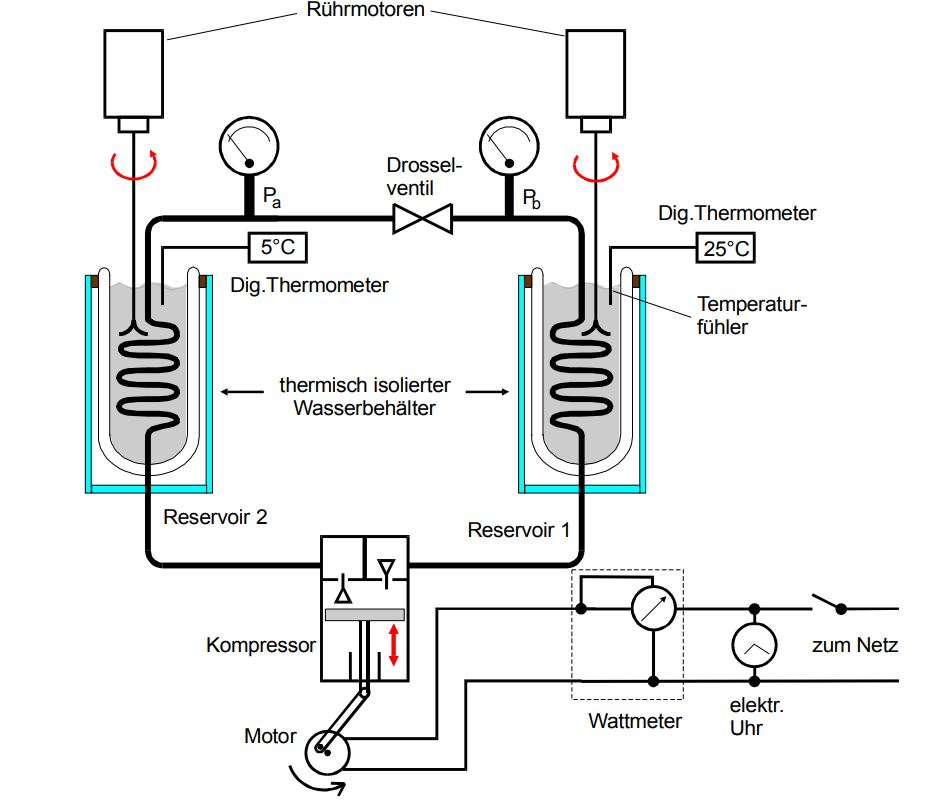
\includegraphics[width=10cm]{content/pumpe.jpg}
% \caption{Schema einer Wärmepumpe}
%   \label{fig:Schema}
%\end{figure}

\noindent\begin{minipage}{0.5\textwidth}
\subsection{Aufbau}
\label{sec:Aufbau}
Hauptbestandteil der Wärmepumpe bilden die zwei Reservoire welche über ein  \\
\textbf{Drosselventil} miteinander Verbunden sind. Jeweils ein \textbf{Druckmessgerät} misst 
den entsprechenden Druck (\textbf{pa, pb}) am Reservoir, welches stets von einem \textbf{Rührmotor} umgedreht wird.
Der steige Durchluss bzw die Pumpfunktion wird gewährleistet durch einen \textbf{Kompressor}, angetrieben durch einen \textbf{Motor}, %steige Durchluss = stetige Durchfluss? :D
 der zwischen die Reservoire gebaut ist. Zum testen der Temperatur liegen digitale 
\textbf{Thermometer} in den isolierten Wasserbehältern.
\end{minipage}
\hfill
\begin{minipage}{0.5\textwidth}\raggedleft
\vspace{2cm}
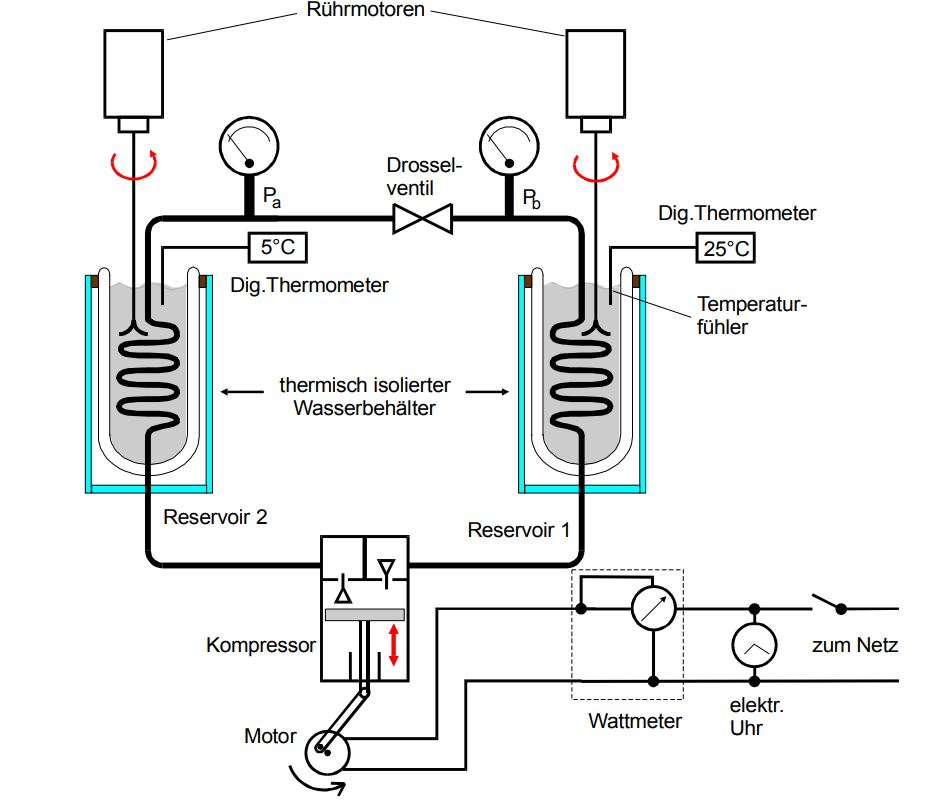
\includegraphics[width=8cm]{content/pumpe.jpg}
\captionof{figure}{Schema einer Wärmepumpe}

\end{minipage}


\subsection{Durchführung}
\label{sec:Durchfuehrung}
Die Wassermengen werden genau abgemessen und in die entsprechenen Rervoire gefüllt. %vllt noch genaue liter angabe
Mit Start des Versuches werden die Temperaturen und Drücke im Absatnd von 1 min von den Anzeigen entnommen. Außerdem wird die vom Wattmeter ausgegebene \textbf{Kompressorleistung} notiert und für 
die Auswertung vorbereitet. Sobald die Temperatur des ersten Rervoire einen Messwert von 50°C erreicht hat, gilt der Verusch als beendet und keine weitern Ergebnisse sind von Interesse.
%vllt noch Transportgas angeben